\documentclass[Protokollheft.tex]{subfiles}
\begin{document}
\chapter{Grundlagen der Methode der Finiten Integration 2}
%--------------- Start Vorbereitungsaufgaben ---------------

\section{Vorbereitungsaufgaben}

% --> Aufgabe
\begin{framed}
	\noindent \textbf{1.} Überlegen Sie sich, wie man ausgehend vom 3-fach Index $i,j,k$ (vgl. Gl.~(3.1)) die Randpunkte eines kartesischen Rechengebietes im kanonischen Indizierungsschema bestimmt (eine Skizze ist hilfreich). Schreiben Sie hierfür ein Schleifenkonstrukt in Pseudocode.\label{exer:boundIdx}
\end{framed}


Randpunkte sind die Punkte, die am Rand des Rechengebietes liegen. Um sie zu finden, sollte man die kanonische Nummerierung und deren Indizies benutzen. Randpunkt ist jeder Punkt, dessen Index ($i,j,k$) gleich 1 oder \lstinline{nx}, \lstinline{ny} beziehungsweise \lstinline{nz} ist. Der Pseudocode, der diese Methode implementiert, ist in Listing 3.1 zu sehen.
\begin{lstlisting}[caption={Pseudocode zur Ermittlung der Randpunkte },label={lst:mgn_RB}]
Randpunkte=[];
Mx=1;
My=nx;
Mz=nx*ny;
kanon=@(i,j,k)(1+(i-1)*Mx+(j-1)*My+(k-1)*Mz);

for i=1:nx
	for j=1:ny
		for k=1:nz
		if i==1 || j==1 || k==1 || i==nx || j==ny || k==nz
		Randpunkte(end+1)=kanon(i,j,k);
		endif
		endfor
	endfor
endfor
\end{lstlisting}
 

% --> Aufgabe
\begin{framed}
	\noindent \textbf{2.} Wie sehen für ein äquidistantes, kartesisches Gitter die Geometriematrizen $\DS$, $\DSd$, $\DA$ und $\DAd$ aus? Was ist bei den Rändern zu beachten? Welche Dimensionen besitzen die Matrizen?\label{exer:geoMatsStructure}
\end{framed}
\noindent
Für ein äquidistantes, kartesisches Gitter bildet die Matrix $\DS$ eine Diagonalmatrix mit dem Abstand $\Delta x$ auf der Diagonalen. Die duale Matrix $\DSd$ unterscheidet sich hiervon nur dadurch, dass die Randelemente mit ½ multipliziert werden. \\
Für die primären Flächen $\DA$ gilt gleichzeitig, dass sie Diagonalmatrizen mit dem Flächeninhalt $\Delta x^2$ sind. Bei der dualen Flächenmatrix $\DAd$ muss nun bei den Randelementen allerdings zwischen, denen, die an einer Randfläche des Rechengebietes liegen und mit ½ multipliziert werden und denen, die an einer Ecke des Rechengebietes die mit ¼ multipliziert werden, unterschieden werden. \\
Falls hier bereits Geisterkanten entfernt worden sind, sind bei den primären Matrizen $\DS$ und $\DA$ die Geisterelemente jeweils Null. \\
\noindent
Die Matrizen besitzen immer die Dimension  $(3np,\ 3np)$ mit $np$ als Anzahl der Gitterpunkte.

% --> Aufgabe
\begin{framed}
	\noindent \textbf{3.} Skizzieren Sie kurz, wie sich die Materialmatrizen zusammenstellen. Wie sind hierbei die Randbedingungen (elektrisch \& magnetisch) einzuarbeiten bzw. muss überhaupt eine Änderung vorgenommen werden?\label{exer:materialMats}
\end{framed}
\noindent
Skizze:\\
$$\Meps =\DAd\Deps\DS^{-1} = \begin{bmatrix}
\tilde{dA}(1) & & \\
& \ddots & \\
& & \tilde{dA}(3\cdot\mathrm{np})
\end{bmatrix}
\cdot
 \begin{bmatrix}
\varepsilon(1) & & \\
& \ddots & \\
& & \varepsilon(3\cdot\mathrm{np})
\end{bmatrix}
\cdot
\begin{bmatrix}
\mathrm{ds}(1) & & \\
& \ddots & \\
& & \mathrm{ds}(3\cdot\mathrm{np})
\end{bmatrix}^{-1}$$
$$\Mmui=\DSd\Dmui\DA^{-1}=
\begin{bmatrix}
\tilde{ds}(1) & & \\
& \ddots & \\
& & \tilde{ds}(3\cdot\mathrm{np})
\end{bmatrix}
\cdot
 \begin{bmatrix}
\mu^{-1}(1) & & \\
& \ddots & \\
& & \mu^{-1}(3\cdot\mathrm{np})
\end{bmatrix}
\cdot
\begin{bmatrix}
\mathrm{dA}(1) & & \\
& \ddots & \\
& & \mathrm{dA}(3\cdot\mathrm{np})
\end{bmatrix}^{-1}$$
\noindent
%Wenn man elektrische Randbedingung hat, muss man die tangentiale Komponente der Permitivität und normale Komponente der Permeabilität am Rand auf Null setzen. Bei magnetischer Randbedingung ist die tangentiale Komponente der magnetischen Feldstärke und normale Komponente des elektrischen Feldes gleich Null. Bei den Materialmatrizen gibt es keine Veränderungen. Die normale Komponente auf dem primären Gitter ist eine Geisterkante und für die Geisterkante ist keine Kante auf dem dualen Gitter definiert. Der Code dazu ist in Listing \ref{lst:mgn_RB} zu sehen.
\noindent
Bei elektrischen Randbedienungen sind die tangentialen Anteile der Permitivität, sowie die normalen Anteile der Permeabilität Null.\\
Bei magnetischen Randbedingungen sind die normalen Anteile des elektrischen Feldes und der tangentiale Anteil des magnetischen Feldes Null. 
Die Materialmatrizen sind hiervon nur indirekt betroffen, da magnetische Randbedingungen automatisch eingepflegt sind. \\
Die normale Komponente auf dem primären Gitter ist eine Geisterkante und für diese ist auf dem dualen Gitter keine Kante definiert. Der Code dazu ist in Listing \ref{lst:mgn_RB} zu sehen.
\begin{lstlisting}[caption={Einsetzen der elektrischen Randbedigungen},label={lst:mgn_RB}]
%% Randbedingungen

% Spezialfall nur bei PEC Rand (bc=1)
if bc==1
 for i=1:nx
  for j=1:ny
   for k=1:nz
    n=1+(i-1)*Mx+(j-1)*My+(k-1)*Mz;
    if k==1 || k==nz
     meanEpsX(n)=0; 
     meanEpsY(n)=0;
    endif
    if j==1 || j==ny
     meanEpsX(n)=0; 
     meanEpsZ(n)=0;
    endif
    if i==1 || i==nx
     meanEpsZ(n)=0; 
     meanEpsY(n)=0;
    endif
   end
  end
 end
end
\end{lstlisting}



% --> Aufgabe
\begin{framed}
	\noindent \textbf{4.} Um die im Versuch zu implementierende Visualisierung zu testen, soll ein vorgegebenes
    rotationssymmetrisches Feld in Zylinderkoordinaten nach der analytischen Formel
    \begin{align}
     \vec{D}(r,\varphi,z)=\frac{1}{r^2} \er
    \end{align}
    visualisiert werden. Es soll ein äquidistantes Gitter benutzt werden, dessen Mitte genau dem Koordinatenursprung entspricht.\\
Bestimmen Sie die diskreten Größen $\dfitloc(n)$ und $\efitloc(n)$ des vorgegebenen Feldes. Zur Vereinfachung soll bei der hierfür notwendigen Integration der Feldwert in der Mitte der Strecke bzw. Fläche als repräsentativ gelten und damit als konstant über dem gesamten Element angenommen werden. \\
    \ \\
    {\textbf{Hinweis:}} Transformieren Sie zuerst zur Bestimmung der notwendigen Feldwerte das gegebene Feld in kartesische Koordinaten $\vec{D}(x,y,z)$.\label{exer:visualizeFieldPrep}
%
\end{framed}
\noindent
Transformiert man $\vec{D}(r,\varphi,z)$ in kartesische Koordinaten ergibt sich
\begin{equation*}
	\vec{D}(x,y,z)=\frac{x}{(x^2+y^2)^{\frac{3}{2}}} \ \vec{e}_x+\frac{y}{(x^2+y^2)^{\frac{3}{2}}} \vec{e}_y.
\end{equation*}
Möchte man nun $\dfitloc(n)$ berechnen muss man einfach $\vec{D}$ am Mittelpunkt der dualen Fläche auswerten und mit dem Flächeninhalt multiplizieren. Um daraus \efitloc(n) zu bestimmt muss einfach die Material Matrix $\Meps$ mit \dfitloc(n) multipliziert werden. Daraus folgt:
\begin{eqnarray*}
\dfitloc(n)&=&\vec{D}(x_n,y_n,z_n)\ \tilde{dA}\\
\efitloc(n)&=&\Meps\dfitloc
\end{eqnarray*}



\section{Aufgaben während der Praktikumssitzung}

\subsection{Materialmatrizen}

% --> Aufgabe
\begin{framed}
	\noindent \textbf{1.} Zuerst sollen zwei Funktionen zum Bestimmen der Geometriematrizen $\DS$, $\DSd$ und $\DA$ geschrieben werden:
\begin{align}
\lstinline{[DS, DSt]} &= \lstinline{createDS(msh)} \label{pro:createDs}\\
\lstinline{[DA]} &= \lstinline{createDA(DS)} \label{pro:createDA}
\end{align}
Wie kann mit der zweiten Funktion auch $\DAd$ bestimmt werden?\label{exer:createDS_DA}
\end{framed}
\noindent
In der Methode \lstinline{createDS} werden die Kantenlängen des Gitters berechnet und als Matrix ausgegeben. Dies geschieht sowohl für das primäre, als auch für das duale Gitter. Dazu kommt die Funktion \lstinline{diff} zum Einsatz. Beim primären Gitter müssen die Geisterkanten zu Null gesetzt werden. Beim dualen Gitter werden die Kanten an den Rändern jeweils halbiert, damit diese nicht herausragen. In der Methode \lstinline{createDA}, in der die Flächen des Gitters berechnet werden können, müssen nun nur noch die richtigen Kantenlängen multipliziert werden.\\
Analog zu $\DA$ kann man die zweite Funktion verwenden, um $\DAd$ zu bestimmen. Dazu muss man nur als Eingabeparameter $\DSd$ setzen.
\begin{align*}
	\lstinline{[DS, DSt]} &= \lstinline{createDS(msh)} \\
	\lstinline{[DAt]} &= \lstinline{createDA(DSt)} 
\end{align*}
% --> Aufgabe
\begin{framed}
	\noindent \textbf{2.} Nun sollen die Funktionen
\begin{align}
\lstinline{[Deps]} &= \lstinline{createDeps(msh, DA, DAt, eps_r, bc)} \label{pro:createDeps}\\
\lstinline{[Meps]} &= \lstinline{createMeps(DAt, Deps, DS)} \label{pro:createMeps}
\end{align}
geschrieben werden, um die $\Meps$-Matrix \lstinline{Meps} aus der $\Deps$-Matrix \lstinline{Deps}
der gemittelten Permittivitäten zu bestimmen.
\lstinline{bc} $=1$ soll dabei elektrische und \lstinline{bc} $=2$ magnetische Randbedingungen bedeuten.
Die Materialverteilung auf dem Gitter \lstinline{msh} soll inhomogen und isotrop bezüglich der Raumrichtungen sein. Zur besseren Übersicht sollen bei der Übergabe relative Permittivitäten verwendet werden. \lstinline{eps_r} soll damit als $N_\text{P}\times 1$ Matrix übergeben werden, also für jedes der $N_\text{P}$ primären Volumen ein $\eps_\text{r}$-Wert.
\\
\textbf{Hinweis:} Für das Invertieren von $\DS$ ist die Methode
\lstinline{nullInv} vorgegeben.\label{exer:createDeps_Meps}
\end{framed}
\noindent
In der Methode \lstinline{createDeps} sollte man sehr vorsichtig mit Randbedingungen und Materialverteilung sein. Bei der Implementierung ist besonders auf die Mittlung an den Rändern zu achten, indem man \lstinline{if}-Bedingungen für die Ränder implementiert. Wenn die Methode \lstinline{createDeps} richtig implementiert wurde, kann man einfach \lstinline{createMeps} mit der bekannten Formel $\Meps=\DAd\Deps\DS^{-1}$ realisieren.
% --> Aufgabe
\begin{framed}
	\noindent \textbf{3.} Die Funktion~\eqref{pro:createMeps} soll nun mit den Parametern
\lstinline{xmesh = [-2 0 2]}, \lstinline{ymesh = [-1 0 1]}, \lstinline{zmesh = [0 1]} und
isotropem $\eps=\eps_0$ die Materialmatrix
$\Meps$ für elektrische Randbedingungen berechnen und ausgeben. Vervollständigen Sie hierfür das bereits gegebene Skript \lstinline{exampleMeps.m}\label{exer:MepsExample}
\end{framed}
\noindent
Durch Ausführen des Skripts \lstinline{exampleMeps.m} erhält man die zwei Diagonalmatrizen $\Deps$ und $\Meps$. Beide Matrizen sind  $54 \times 54$ Matrizen. 


\subsection{Interpolation und Visualisierung}

% --> Aufgabe
\begin{framed}
	\noindent \textbf{4.} Programmieren Sie eine Routine
\begin{align}
	\lstinline{eField = fitInt(msh, eBow)} \; , \label{mthd:fitInt}
\end{align}	
die die Komponenten von $\efit$ als $\vec{E}$-Feld auf die primären Punkte interpoliert.\label{exer:fitInt}
\end{framed}
\noindent
Zur Verbesserung der Laufzeit werden die Interpolationen als Matrixoperationen und nicht als Schleifen ausgeführt. Hierzu werden Verschiebungsmatritzen erstellt um damit durch Multiplikation 
\begin{equation*}
	e_x(P(n)) =\frac{e_x (n - M_x )\Delta x(n) + e_x (n)\Delta x(n - M_x)}  {\Delta x(n - M_x ) + \Delta x(n)}
\end{equation*} 
 zu berechnen.


% --> Aufgabe
\begin{framed}
	\noindent \textbf{5.} Schreiben sie eine Methode
\begin{align}
	\lstinline{plotEBow(msh, eBow, indz)} \; , \label{mthd:plotEBow}
\end{align}
die auf Methode~\eqref{mthd:fitInt} aufbauend $\efit$ interpoliert und den
Betrag des $\vec{E}$-Feldes mit dem \matlab-Befehl \lstinline{surf} in einer
$x$-$y$-Ebene mit Index \lstinline{indz} grafisch darstellt. Verwenden Sie hierfür bitte elektrische Randbedingungen.
\\
\textbf{Hinweis:} Nutzen Sie auch für das Invertieren von $\Meps$ die vorgegebene Methode
\lstinline{nullInv}.\label{exer:plotEBow}
\end{framed}
\noindent
Die Methode \lstinline{plotEBow} lässt sich mit wenigen Operationen implementieren.
Zunächst wird der Vektor \lstinline{eBow} in die Anteile in $x$-, $y$- und $z$-Richtung zerlegt. Danach wird mit diesen Angaben der Betrag des Feldes an jeder Stelle berechnet. Durch nun einfaches Auswählen des gewünschten Bereiches mit \lstinline{indz} kann nun das elektrische Feld grafisch dargestellt werden.


% --> Aufgabe
\begin{framed}
	\noindent \textbf{6.} Geben Sie das rotationssymmetrische Feld aus der Vorbereitung als
Vektor $\dfit$ vor, berechnen Sie daraus mit Hilfe der Materialmatrix $\Mepsi$
das Feld $\efit$ und wenden Sie dann Methode \eqref{mthd:plotEBow} an. Visualisieren Sie außerdem die selbe Schnittebene mit der in Versuch 2 vorgestellten Methode \lstinline{plotEdgeVoltage}. Vervollständigen Sie hierfür den ersten Teil des bereits gegebenen Skripts \lstinline{exampleVisualEfield.m}\label{exer:exampleVisualEfield1}
\end{framed}
\noindent
Das elektrische Feld für isotrope Materialien ist in den Abbildungen \ref{Abb:61} und \ref{Abb:62} dargestellt.

% --> Aufgabe
\begin{framed}
	\noindent \textbf{7.} Überlegen Sie sich, welche Änderungen an den bisher implementierten Methoden 
vorgenommen werden müssen, um ein anisotropes Material zu verwenden. Ändern Sie 
Ihre Implementierung entsprechend und verwenden Sie ein anisotropes Material mit unterschiedlichen
Permittivitäten in $x$- und $y$-Richtung (z.\,B.
$\eps_x / \eps_y=4$) sowie elektrische
Randbedingungen. Interpolieren und visualisieren Sie das Feld
$\efit$ wie in der Aufgabe zuvor. Visualisieren Sie auch hier das Ergebnis zusätzlich mit der Methode \lstinline{plotEdgeVoltage}. Vervollständigen Sie hierfür den zweiten Teil des bereits gegebenen Skripts \lstinline{exampleVisualEfield.m}\label{exer:exampleVisualEfield2}\\
\end{framed}
\noindent
Für anisotrope Materialien muss die Methode \lstinline{createDeps.m} so angepasst werden, dass der Vektor \lstinline{eps_r} auch die Läange $3n_p$ besitzen darf. Das elektrische Feld für anisotrope Materialien ist in den Abbildungen \ref{Abb:71} und \ref{Abb:72} dargestellt.

\section{Fragen zur Ausarbeitung}

% --> Aufgabe
	\begin{framed}
	\noindent \textbf{1.} Erstellen Sie eine 2D-Skizze einer dualen
	Gitterfläche mit den zugehörigen primären Gitterzellen, welche
    zur Mittelung der Permittivität notwendig sind (siehe (3.10)).\label{exer:averagingEps}
\end{framed}
\noindent
Die duale Fläche mit den zugehörigen primären Gitterzellen sind in Abbildung \ref{Abb:A1} zu sehen. Die duale Fläche $\tilde{A}$ liegt auf der Mitte der Länge der primalen Kante $L_1$. $\tilde{A}$ teilt sich auf alle 4 anliegenden primären Volumen auf.


% --> Aufgabe
	\begin{framed}
	\noindent \textbf{2.} Häufig werden für die Visualisierung der magnetischen Feldstärke
	$\Hv$ die entsprechenden Komponenten ebenfalls auf den Punkten des
	primären Gitters gemittelt und nicht auf den dualen
	Punkten. Beschreiben Sie für diese Mittelung \emph{kurz} eine geeignete Vorgehensweise (kleine Skizze sinnvoll)
	und gehen Sie dabei auch auf die Randbedingungen ein.\label{exer:averageHfield}
\end{framed}
\noindent
Für die Mittelung von $\Hv$ auf den Primären Punkten muss zunächst die magnetische Flussdichte $\vec{B}$ von den 4 anliegenden primären Flächen mit $\bar{B}=\frac{1}{4}(B_1+B_2+B_3+B_4)$ gemittelt werden. Nun muss man weiterhin die Materialkonstate $\mu$ über die 8 anliegenden primären Volumen mit $\bar{\mu}=\frac{1}{8}(\mu_1+\mu_2+\mu_3+\mu_4+\mu_5+\mu_6+\mu_7+\mu_8)$ mitteln. Die Feldstärke $\Hv$ ergibt sich nun aus der Materialbeziehung zwischen $\vec{B}$ und $\Hv$. Damit erhalten wir $\Hv=\bar{\mu}\bar{B}$. Eine Darstellung ist in Abbildung \ref{Abb:A2} zu sehen.

\section{Fazit}
Wie in der Ausarbeitung deutlich wird, ist es nun möglich Materialmatrizen zu erstellen, sowie elektrische Felder zu visualisieren.

\section{Abbildungen}
\begin{figure}[h!]
	\centering
	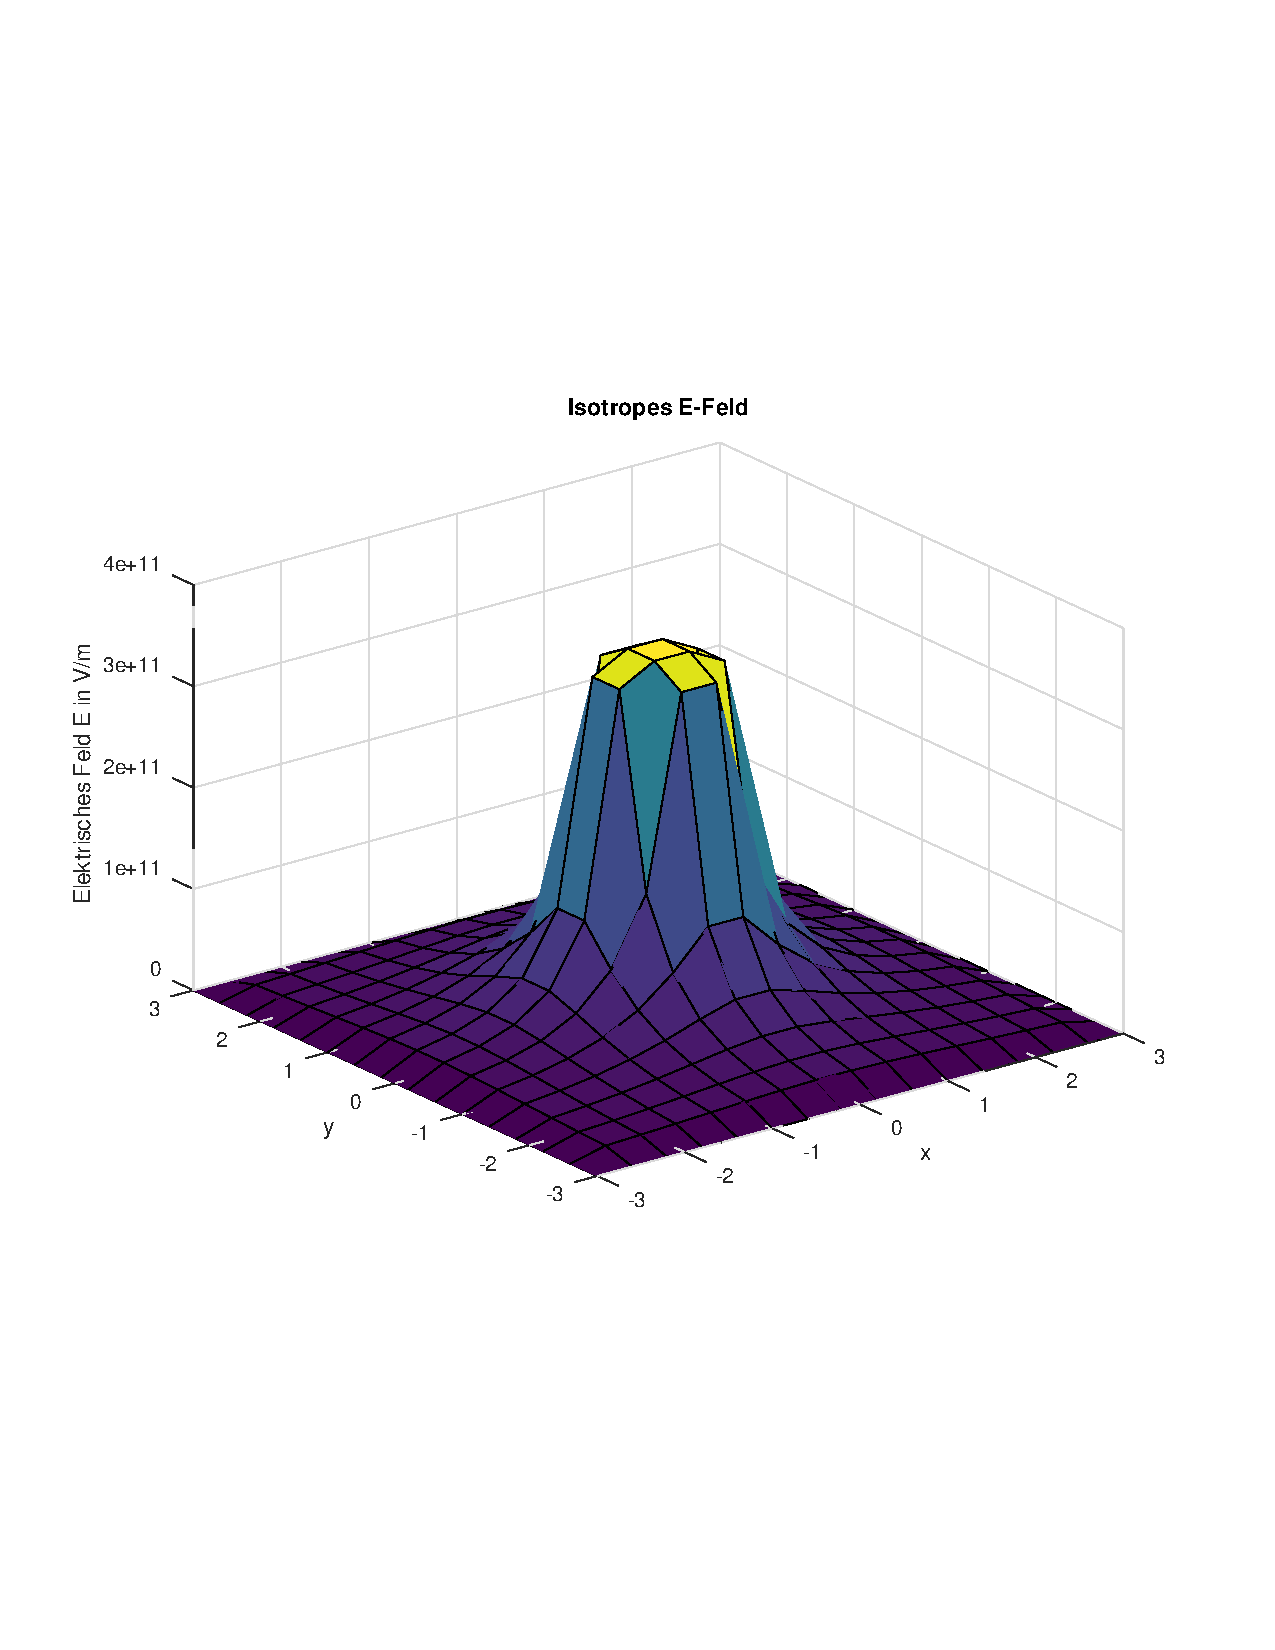
\includegraphics[trim = 10mm 60mm 10mm 50mm, clip, width=0.7\textwidth]{efield_1.pdf}
	\caption{Elektrisches Feld bei isotroper Materialverteilung in 3D.}
	\label{Abb:61}
\end{figure}

\begin{figure}[h!]
	\centering
	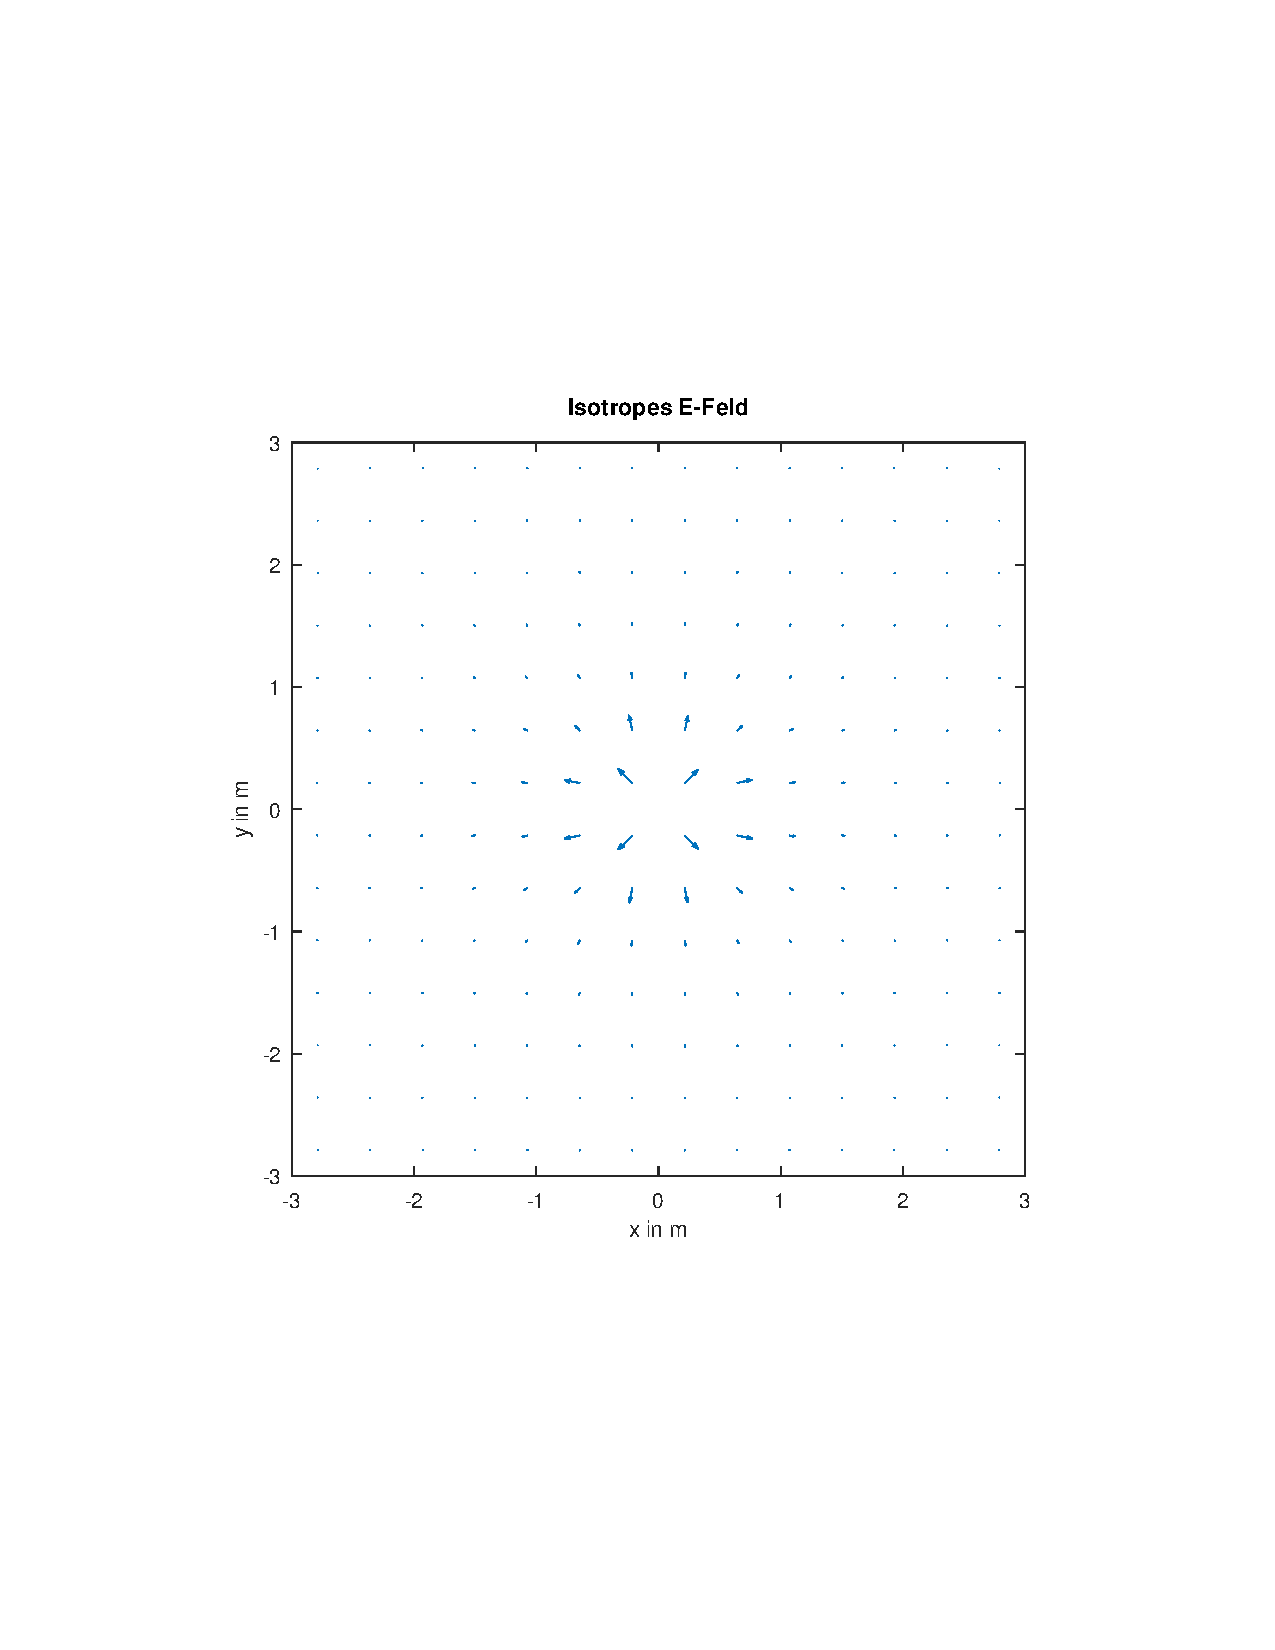
\includegraphics[trim = 10mm 60mm 10mm 50mm, clip, width=0.7\textwidth]{efield_2.pdf}
	\caption{Elektrisches Feld bei isotroper Materialverteilung dargestellt mit Vektorpfeilen.}
	\label{Abb:62}
\end{figure}
\begin{figure}[h!]
	\centering
	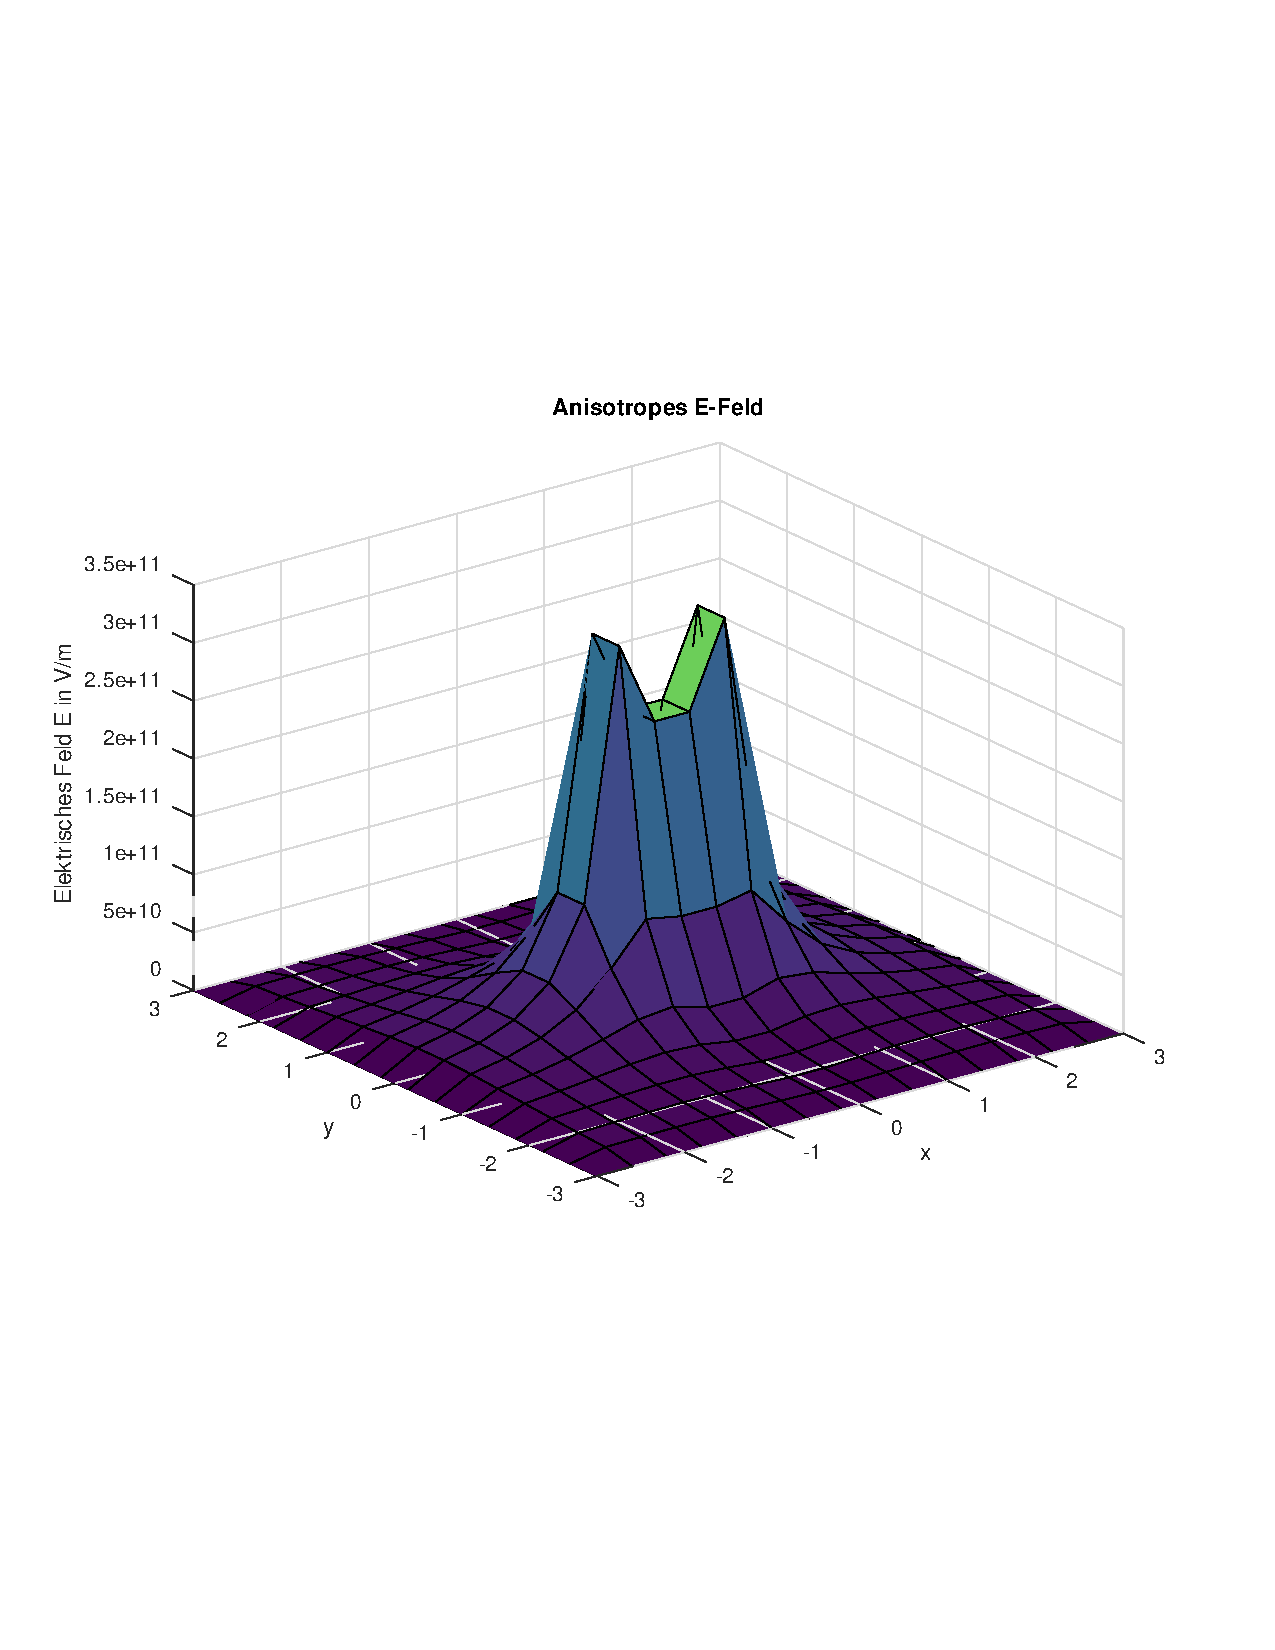
\includegraphics[trim = 10mm 60mm 10mm 50mm, clip, width=0.7\textwidth]{efield_3.pdf}
	\caption{Elektrisches Feld bei anisotroper Materialverteilung in 3D.}
	\label{Abb:71}
\end{figure}

\begin{figure}[h!]
	\centering
	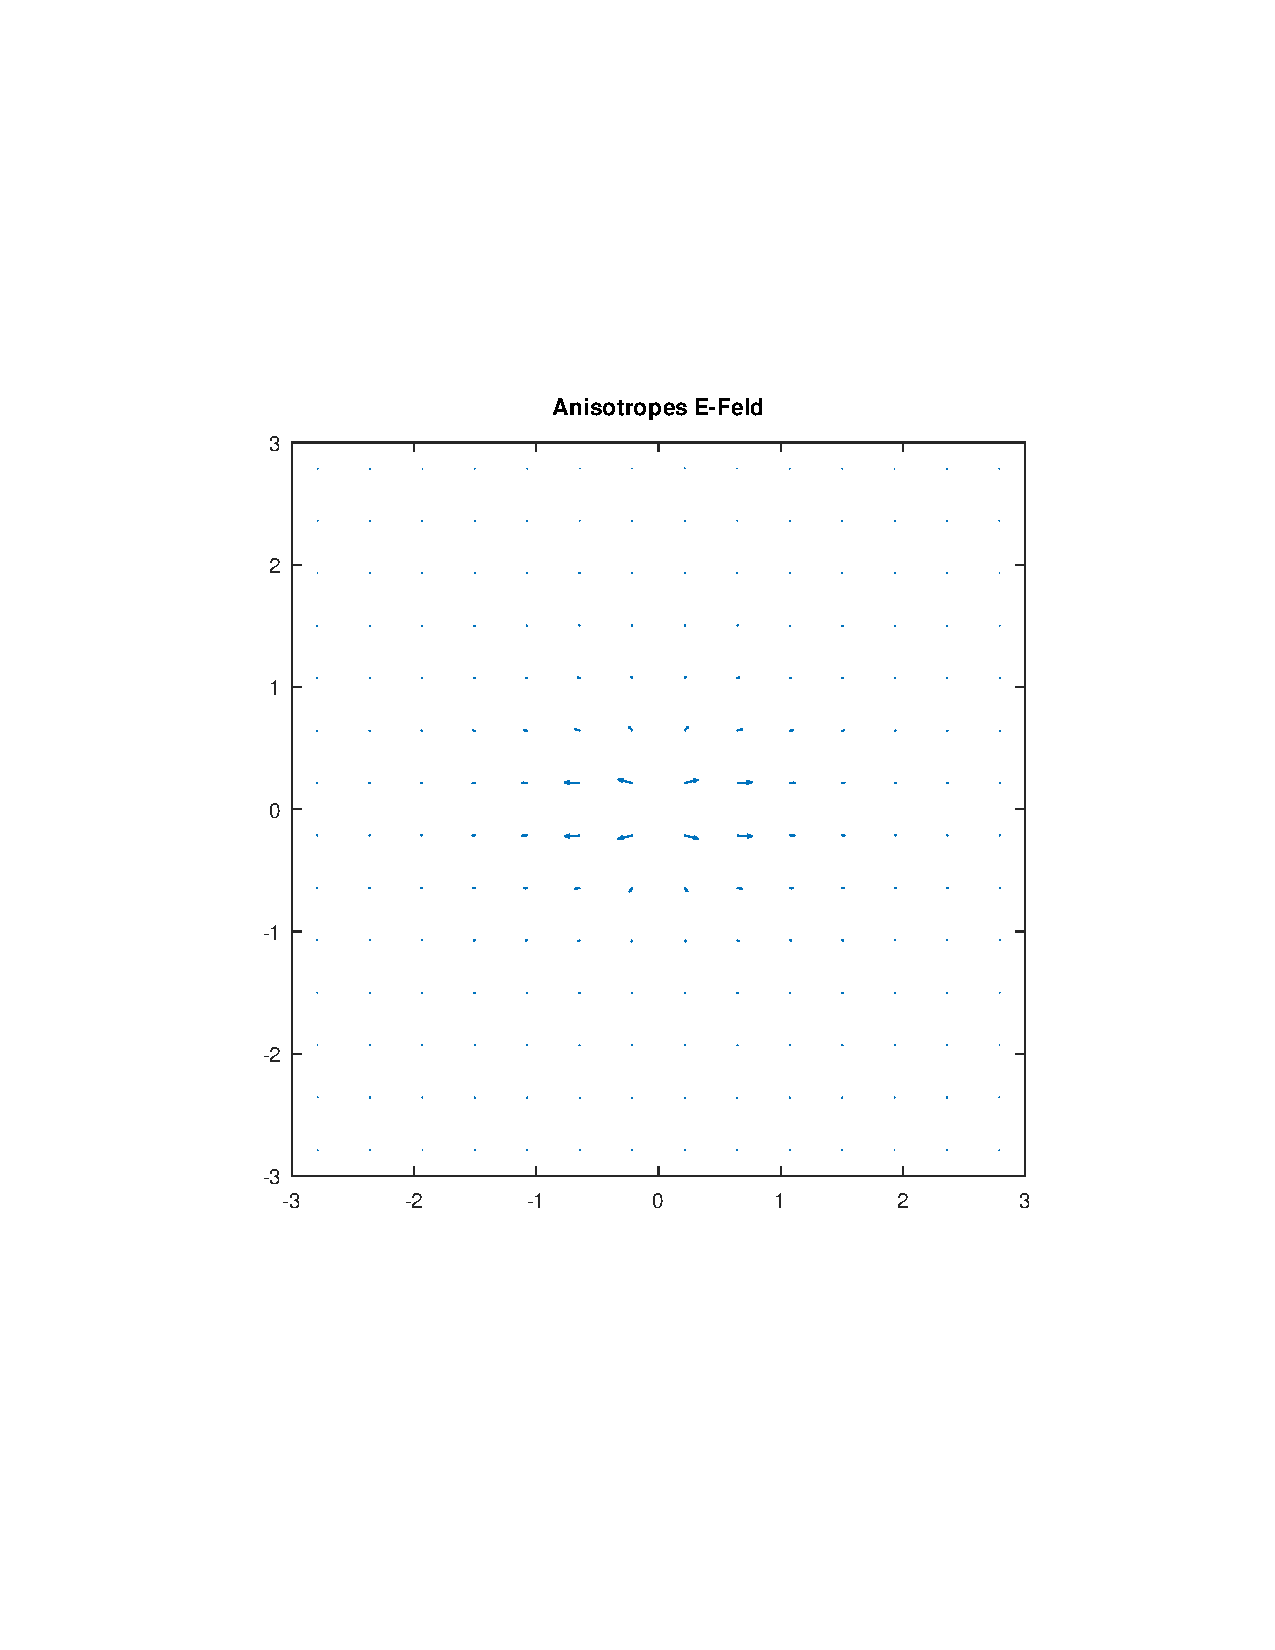
\includegraphics[trim = 10mm 60mm 10mm 50mm, clip, width=0.7\textwidth]{efield_4.pdf}
	\caption{Elektrisches Feld bei anisotroper Materialverteilung dargestellt mit Vektorpfeilen.}
	\label{Abb:72}
\end{figure}
\begin{figure}[h!]
	\centering
	\def\svgwidth{0.5\textwidth}
	\input{versuch3/dual_flaeche.pdf_tex}
	\caption{Duale Fläche (Mitte) mit den primären Gitterzellen. Die für die Mittelung interessanten Bereiche sind schraffiert.}
	\label{Abb:A1}
\end{figure}
\begin{figure}[h!]
	\centering
	\def\svgwidth{0.5\textwidth}
	\input{versuch3/b_h_mitt.pdf_tex}
	\caption{Darstellung der örtlichen Beziehungen zwischen $\Hv$ und $\vec{B}$.}
	\label{Abb:A2}
\end{figure}

\end{document}
